\section{Collision Avoidance} \label{sec:collision_avoidance}

\subsection{Disturbance Repulsion}
A crucial property of the passive obstacle-aware controller is its ability to ensure collision avoidance. For this, we analyze the ability and limitations of the proposed controller to absorb disturbances.
Let us assume a disturbance impact at time $t=0$, which results in the robot having a velocity of $\vecs{\dot \xi} = \vect f(\vecs \xi) + \vect v^I$, which is pointing towards the obstacle (see Fig.~\ref{fig:disturbance_with_parallel_velocity}). 
Note that, the Coriolis effect is neglected due to the small motion of the agent.

\begin{lemma}
	Let us consider a dynamical system that evolves according to the rigid body dynamics given in \eqref{eq:robot_dynamics} and is governed by the obstacle aware, passive controller \eqref{eq:control_command}, using the damping matrix $\matd{D}$ as defined in \eqref{eq:damping_summation}, and neglectable Coriolis effect.
    An agent moving close to the surface, i.e., $\Gamma(\vecs \xi) \approx 1$ is disturbed by a large disturbance velocity $v^I$ compared to the initial velocity, i.e., $\| \vect f(\vecs \xi) \| / \|\vect v^I \| \ll 1 $.
	The motion starting in free space, i.e., $\Gamma( \{\vecs \xi_0 \} ) > 1$ is able to reject the disturbance and remain collision-free for all times $\Gamma( \{\vecs \xi_t\}) \geq 1$ with $t \geq 0$ if the impact velocity is limited as follows $\| \vect v^I \| < s^{\mathrm{o}} \| \vecs \xi - \vecs \xi^b \| / m^{\mathrm{min}}$, with respect to the closes surface point $\vecs \xi^b \in \mathbb{R}^N$ and smallest eigenvalue of the mass matrix $m^{\mathrm{min}} \in \mathbb{R}_{>0}$.
\end{lemma}


\begin{figure}[htb]
\centering
 % \begin{subfigure}{0.99\columnwidth}
  \centerline{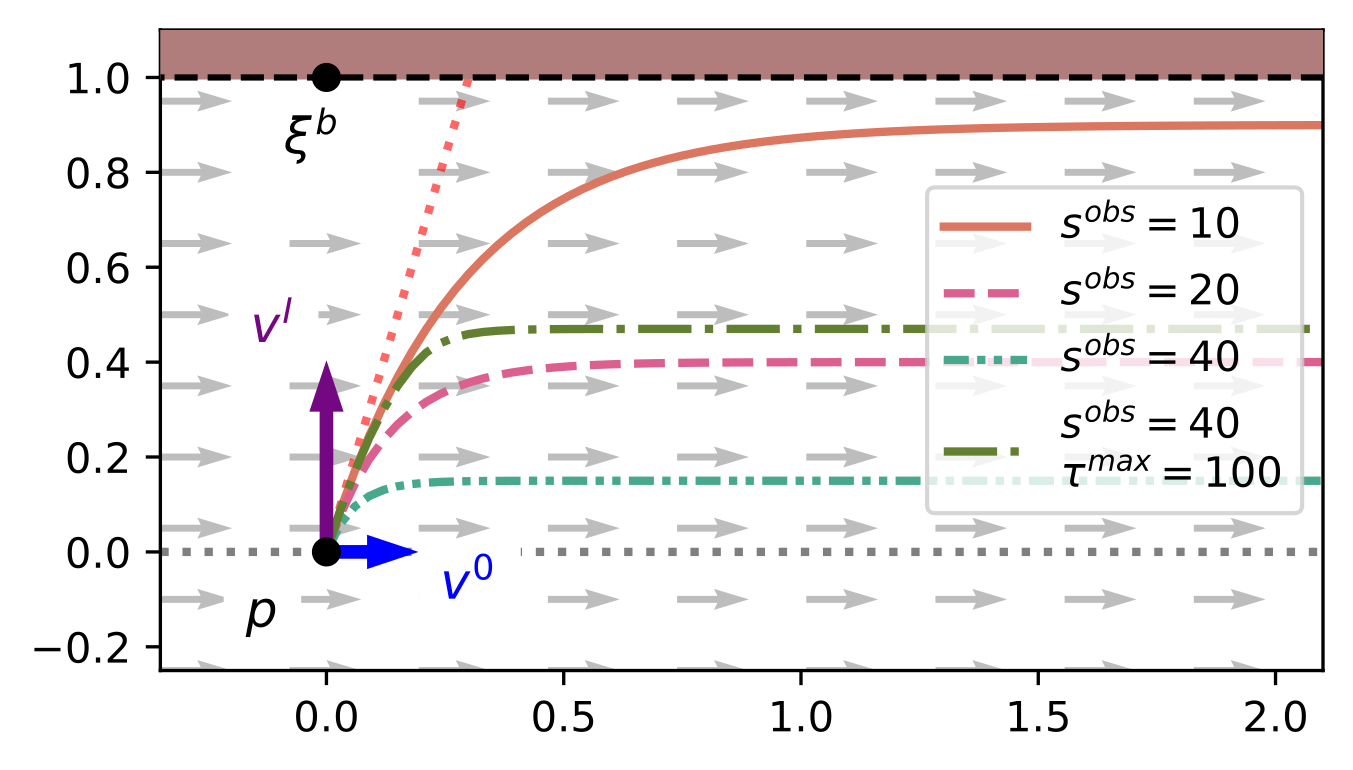
\includegraphics[width=0.99\columnwidth]{figures/parallel_avoidance_obstacle}}
  \caption{Disturbance rejection in the presence of a constant velocity field (blue), and different damping values $s^{\mathrm{obs}}$ and optionally a maximum repulsion force $\vecs \tau^{\mathrm{max}}$ for the green trajectory.}
  \label{fig:disturbance_with_parallel_velocity}
% \end{subfigure}
\end{figure}

\begin{proof}
Using \eqref{eq:control_command}, the velocity is evaluated as follows:
\begin{equation}
\begin{split}
    \vecs{\dot \xi} & = \int \vecs{\ddot \xi} \, dt 
    = \int \matd{M}^{-1} \matd{D}  \left( \vecs{\dot \xi} - \vecs f(\vecs \xi) \right) \, dt \\
    & \approx \int \matd{M}^{-1} \matd{D} \vecs{\dot \xi} \, dt
\end{split}
\end{equation}
where we use the approximation, of the disturbance velocity being high, i.e., $\| \vect f(\vecs \xi) \| / \|\vect v^I \| \approx 0 $, 

Due to the proximity to the obstacle, the danger weight in \eqref{eq:weight_function} is evaluated as $w(\vecs \xi) \approx 1$, and the damping in the direction of the obstacle from \eqref{eq:damping_summation} is approximated as $s^{\mathrm{obs}}$. 
Hence, the most critical scenario is when the disturbance is directly toward the obstacle. A general velocity evolution towards the obstacle is smaller than this.
Hence, we focus on this extreme case:
\begin{equation}
    \vecs{\dot \xi} = \int \frac{s^{\mathrm{o}}}{m} \vecs{ \dot \xi} \, dt = \frac{s^{\mathrm{o}}}{m} (\vecs{\xi} - \vecs \xi_0)  + \vecs v^I \label{eq:velocity_with_control}
\end{equation}
where $m = \min \Bigl(\text{eig} \bigl(\mathcal{M} \bigr) \Bigr)$ is the smallest eigenvalue of the mass matrix. Note, that any velocity which does not point towards the surface, will not get as close to the obstacle.

This can be used to compute the distance at which the velocity reaches zero:
\begin{equation}
    \| \vecs{\dot \xi} \| = 0
    \quad \Rightarrow \quad
    \|\vecs \xi_0 - \vecs{\xi} \| = \| \vecs v^I \| {m} / {s^{\mathrm{o}}} 
\end{equation}
where $\vecs \xi_0 \in \mathbb{R}^N $ is the starting position. 

Hence, if the disturbance velocity is limited by 
\begin{equation}
    \| \vect v^I \| < s^{\mathrm{o}} \| \vecs \xi - \vecs \xi^b \| / m
\end{equation}
with respect to the closes surface point $\vecs \xi^b \in \mathbb{R}^N$ and smallest eigenvalue of the mass matrix $m$.
\end{proof}

Note that the analysis is done for proximity regions of the obstacle. In any case, the robot enters this proximity region before a collision can occur. Hence, the proposed analysis holds as a general collision avoidance insurance.

So far the disturbance has been in the form of a velocity, yet a system is disturbed by force. The corresponding disturbance velocity is obtained by integrating the force over time (considering the mass matrix). 

\subsection{Disturbance Repulsion with Force Limit}
All robotic systems have a maximum force that they  exert based on the motors and their geometry, $\tau_c^{\mathrm{max}} \in \mathbb{R}_{>0}$. Note that such a force might be state-dependent.

A limiting force increases the impact velocity $\vect v^I$ a controller can handle to ensure collision avoidance (Fig.~\ref{fig:disturbance_with_parallel_velocity}). Nevertheless, a maximum control force can be interpreted as an adapting damping parameter, and hence, the passivity from Theorem~\ref{theorem:passivity} still holds.


